\footnote{\cite{allendorf2013going} used a sample of married women age 15 -- 29, rather than pregnant women in particular.  To check the appropriateness of the comparison, Appendix Figure C-3 shows that if we use \cite{allendorf2012women}'s sample and the time period this paper studies, we find a decrease in patrilocal extended households.  Indeed, in the same group that \cite{allendorf2013going} studied, patrilocal extended family residence decreased from 41\% in 2005--2006 to 31\% in 2019--2021.} 

Figure \ref{fig:allendorf} shows changes in the distribution of household structure among married women aged 15–29 who are living with their husband and are usual residents of their household. These are similar sample restrictions as used in \cite{allendorf2013going}, which found increasing nuclear residence between 1992 and 2006. In this sample as well, we find increasing patrilocal residence between 2005 and 2021, a reversal of the trend documented by \cite{allendorf2013going}. In fact, the share of women living in patrilocal households is higher in 2019--2021 than it was as \cite{allendorf2013going} found in 1992--1993. 


\begin{figure}[H]
\begin{flushleft}
\caption{: Trends in household structure among married women aged 15--29 who are living with their husband and are usual residents of their household.}
\vspace{0em}
\label{fig:allendorf}
\begin{center}
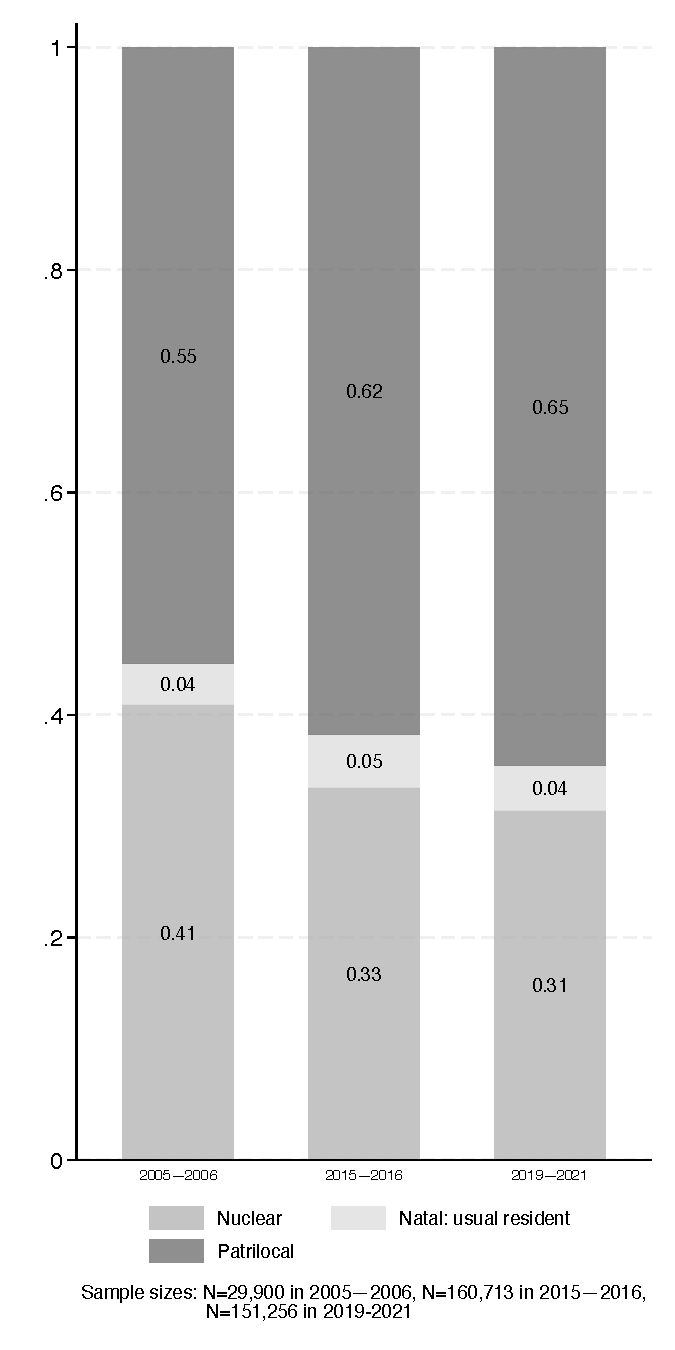
\includegraphics[width=0.4\textwidth]{figures/figureC3_hhstruc_composition_allendorf2013sample.pdf}
\end{center}

\vspace{1ex}
\small\scriptsize{\textsf{\textit{Note}: Data are from NFHS rounds 3 (2005--2006), 4 (2015--2016), and 5 (2019--2021). The sample is restricted to married women between the ages of 15--29 who are usual residents of either a nuclear, patrilocal, or natal household, and are currently living with their husband. \cite{allendorf2013going} found rising nuclearization in NFHS 1 (1992-1993), 2 (1998-1999), and 3 (2005--2006) data using the same sample restrictions in addition to restricting for only women in nuclear or patrilocal households.}}
\end{flushleft}
\end{figure}


\section*{Abstract}
Research on young women in India that studies the 1990s to the early 2000s documents a shift away from patrilocal extended family residence towards nuclear households, and suggests trade-offs between women’s autonomy and access to resources across household types.  Our descriptive analysis uses three rounds of the National Family Health Surveys to show that between 2005 and 2021, pregnant women increasingly lived in patrilocal extended households.  This may be surprising to researchers who associate increasing modernization with nuclear family structures.  To understand the ramifications of this trend, we compare pregnant women’s autonomy and healthcare use across household types and assess changes in these relationships over time.  We find that, over this period, pregnant women in extended households have less decision-making power and more healthcare use than those in nuclear households, but that these differences are shrinking over time. Our results speak to a growing literature on demographic change in India: the trend towards pregnancy and parenthood occurring in extended families may continue as grandparents live longer and successive generations have smaller families, but may not have the consequences implied by the prior literature on family structure.